\chapter{Recommended Procedures for Developing Test Cases}

In addition to the Test Cases themselves, the learnings from developing the Test Cases is presented.  This will both help the reader understand why the particular Test Cases were chosen and provide a methodology for developing any new cases.


Drill string models are complex and contain a number of parameters.  These parameters are used to make a simulation more realistic, but they are often implemented in different ways in different models.



\begin{bulletedlist}
	\item For initial model comparison, remove top drive to eliminate it as a variable
	\item Use with a vertical borehole

	\item Note how tool joints are handled: ignored, modified stiffness (equivalent stiffness), account for contact/friction?
	\item Carefully examine the units and ensure they are accurately converted
\end{bulletedlist}
\notfinished{}

\section{Friction Models}
When working with various friction models, it becomes vital to identify parameters that result in similar frictional behaviors.  The parameters for the friction models are static coefficient of friction, dynamic coefficient of friction, and critical velocity. Generally, the static and dynamic coefficients of friction can be equated across different models, while special attention is required to align the critical velocity with the desired frictional behavior.

\subsection{Units}
In the context of modeling torsional dynamics, if the critical velocities of two different models are provided in different units such as meters per second ($m/s$) and revolutions per minute ($RPM$), unit compatibility must first be established for meaningful comparison. Converting $m/s$ to $RPM$ can be achieved by \equationname~\ref{velocity_conversion}.
\begin{equation}\label{velocity_conversion}
  V=v\frac{60}{2\pi}*r_o
\end{equation}
where $V$ and $v$ are angular velocity expressed in $RPM$, and $m/s$, respectively, and $r_o$ is outer radius of the drill pipe.  Note that this conversion relies on the pipe diameter and thus will, in general, vary along the length of the drill string.  For this reason, it is preferred that the input units for the critical velocity to be linear and the conversion be done internally by the drill string model on each pipe segment.



% \wordingstart{} After matching the units, the critical angular velocity of the model, which is for the comparison, can be decided by comparing the frictional force with respect to angular velocity. \wordingend{}
%For instance, considering Test Case 2 with a critical velocity of 0.03 $m/s$ and a drill string radius of 0.075 $m$, the critical velocity can be converted to 4$RPM$.

\figurename~\ref{figure:stribeck_coulomb_friction} shows an example comparison between Coulomb and Stribeck friction models. It compares two different critical velocities of a Coulomb model with a Stribeck model.

In this project, we selected an angular velocity of 10 $RPM$ for the Coulomb model. This choice allows us to align the exponentially decreasing component of the Stribeck model with the static friction inherent in the Coulomb friction model. However, it is important to note that additional tests involving different angular velocities have been performed and are included in the appendix chapter for comprehensive analysis. \reviewcomment{If not added, modify}

\begin{figure}
  \centering
  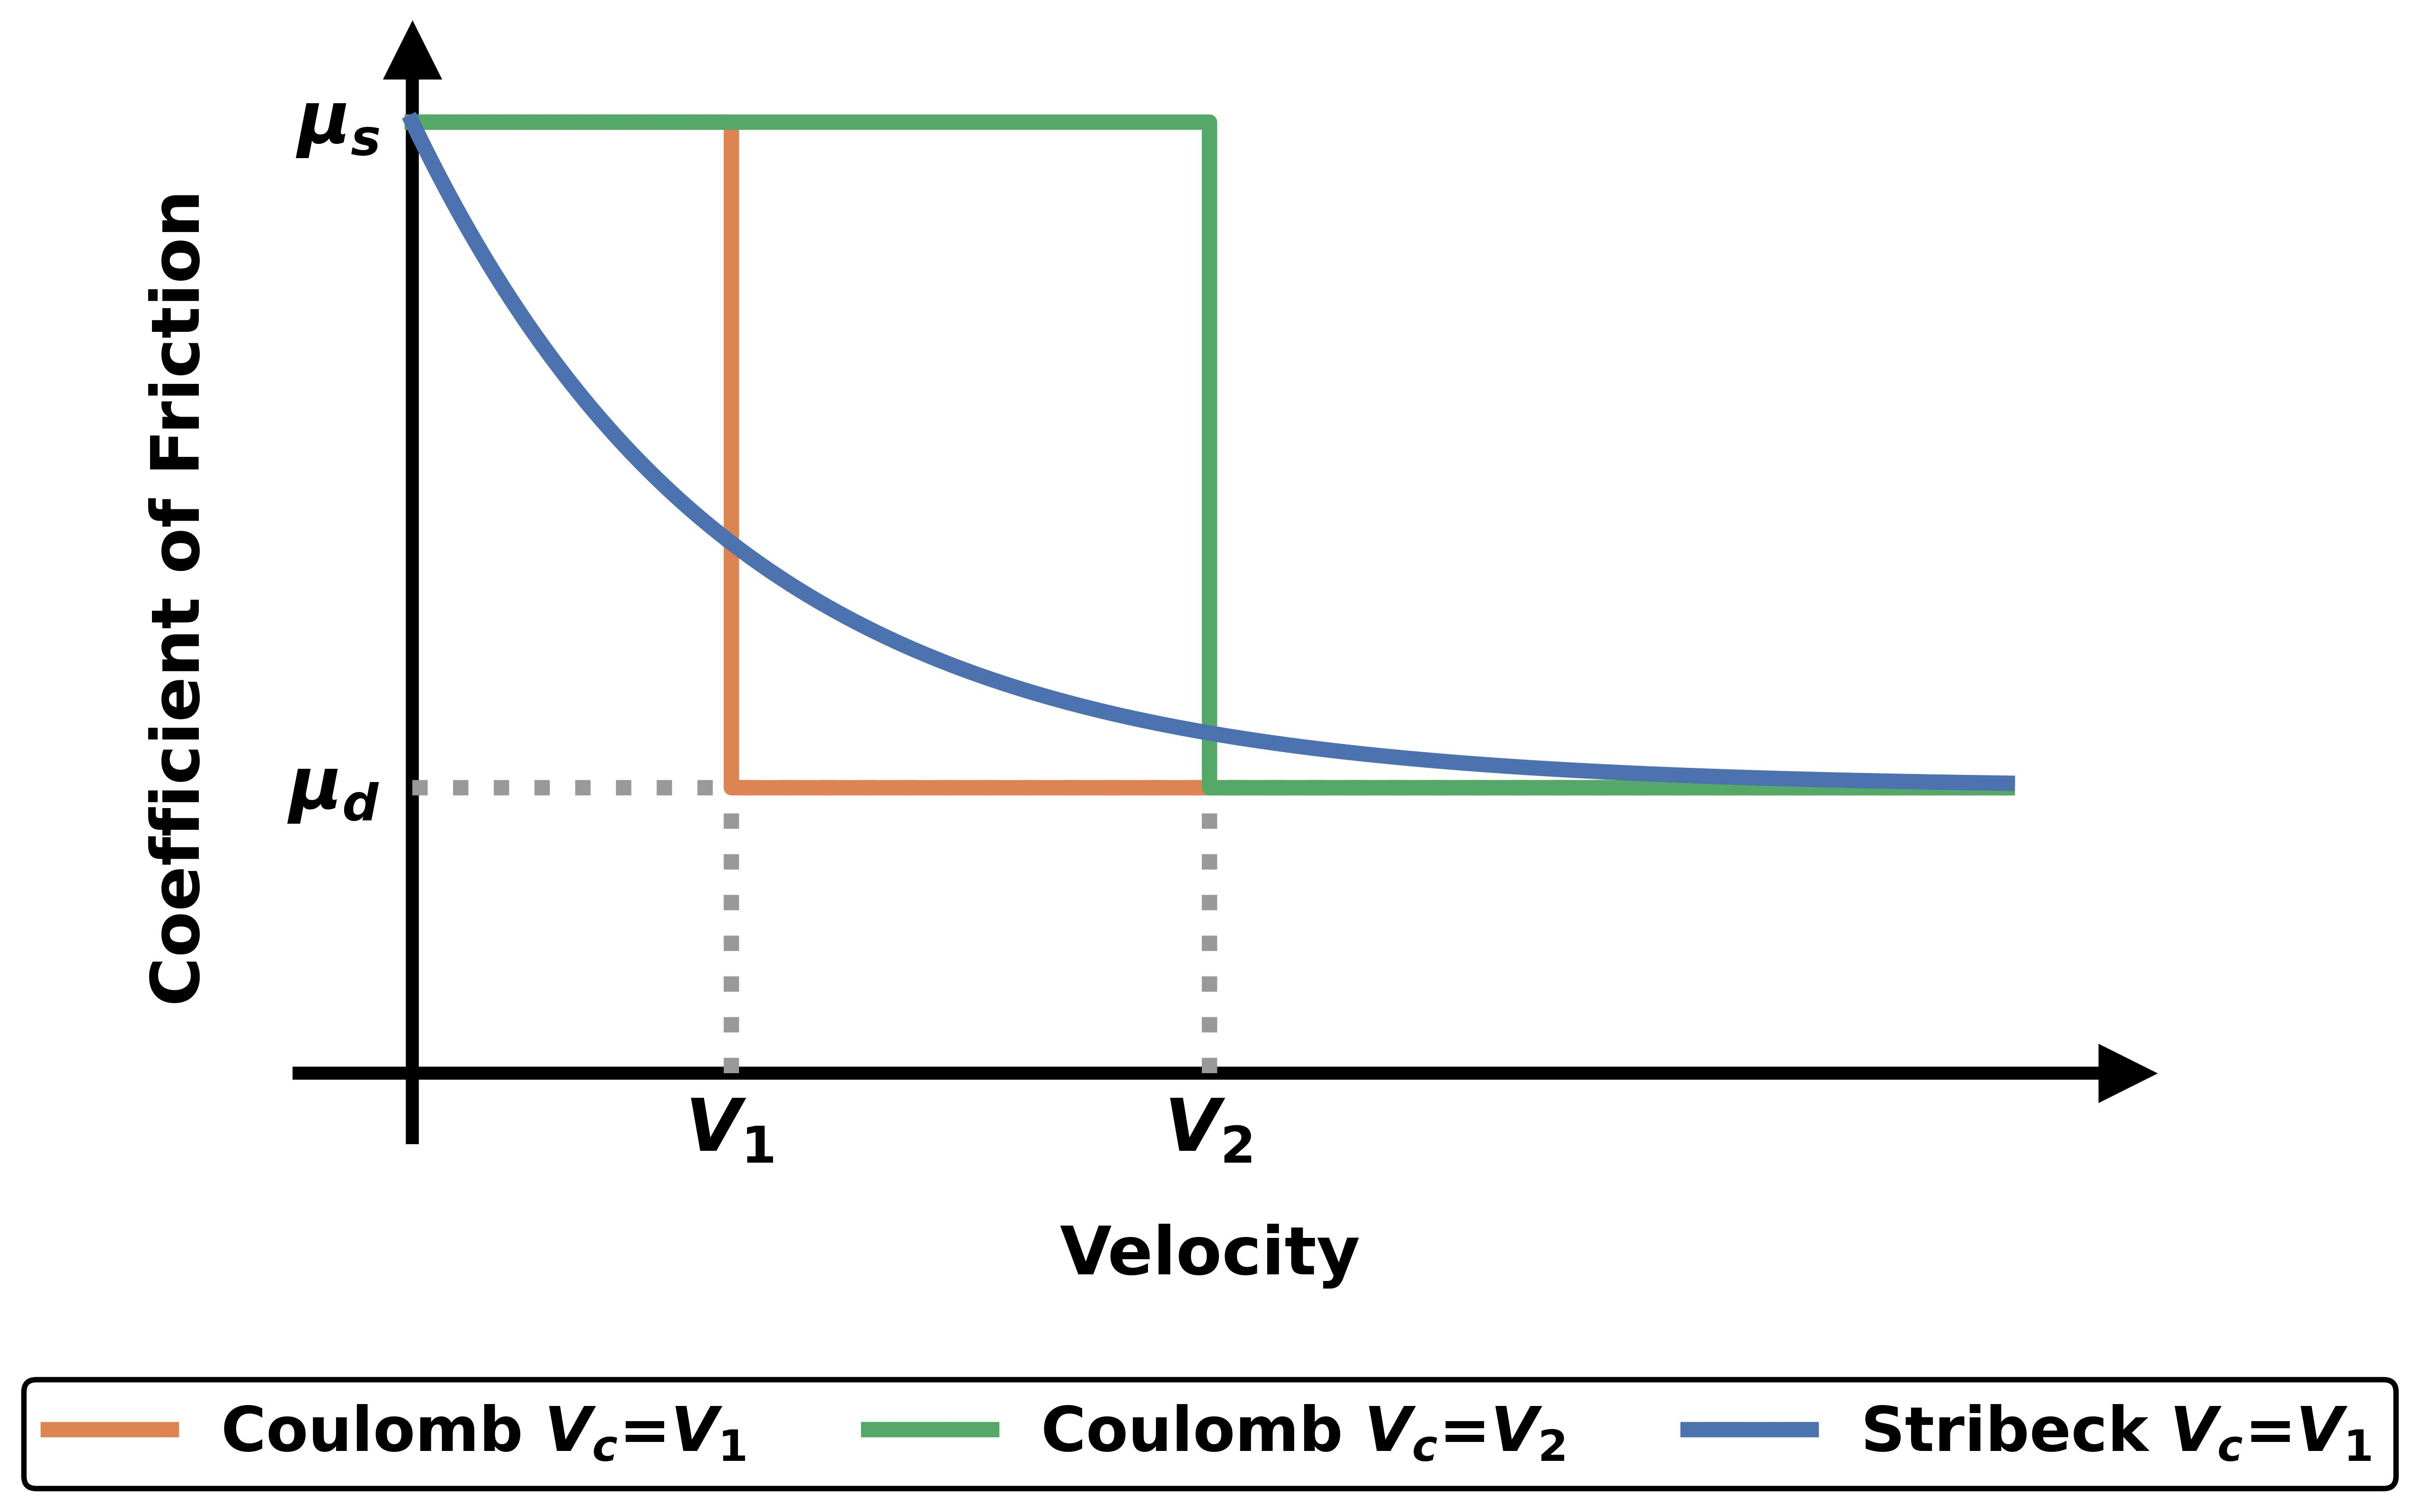
\includegraphics[width=5in]{Stribeck_Coulomb_friction}
  \caption[Comparison between Coulomb and Stribeck friction model]{A comparison between Coulomb and Stribeck friction models. A Stribeck model with a critical velocity of $V_1$ is compared to Coulomb friction models with critical velocities of $V_1$ and $V_2$. $\mu_s$ and $\mu_d$ indicate the static and dynamic coefficients of friction, respectively, and $V$ is the velocity.  The Coulomb model with a critical velocity of $V_1$ matches the critical velocity of the Stribeck friction.  The choice of $V_2$ as the critical velocity for the Coulomb friction is closer to the point where the Stribeck model coefficient begins to significantly increase.}\label{figure:stribeck_coulomb_friction}
\end{figure}

\begin{figure}
	\begin{minipage}[t]{\linewidth}
			\begin{minipage}[t]{0.325\linewidth}
				\centering
				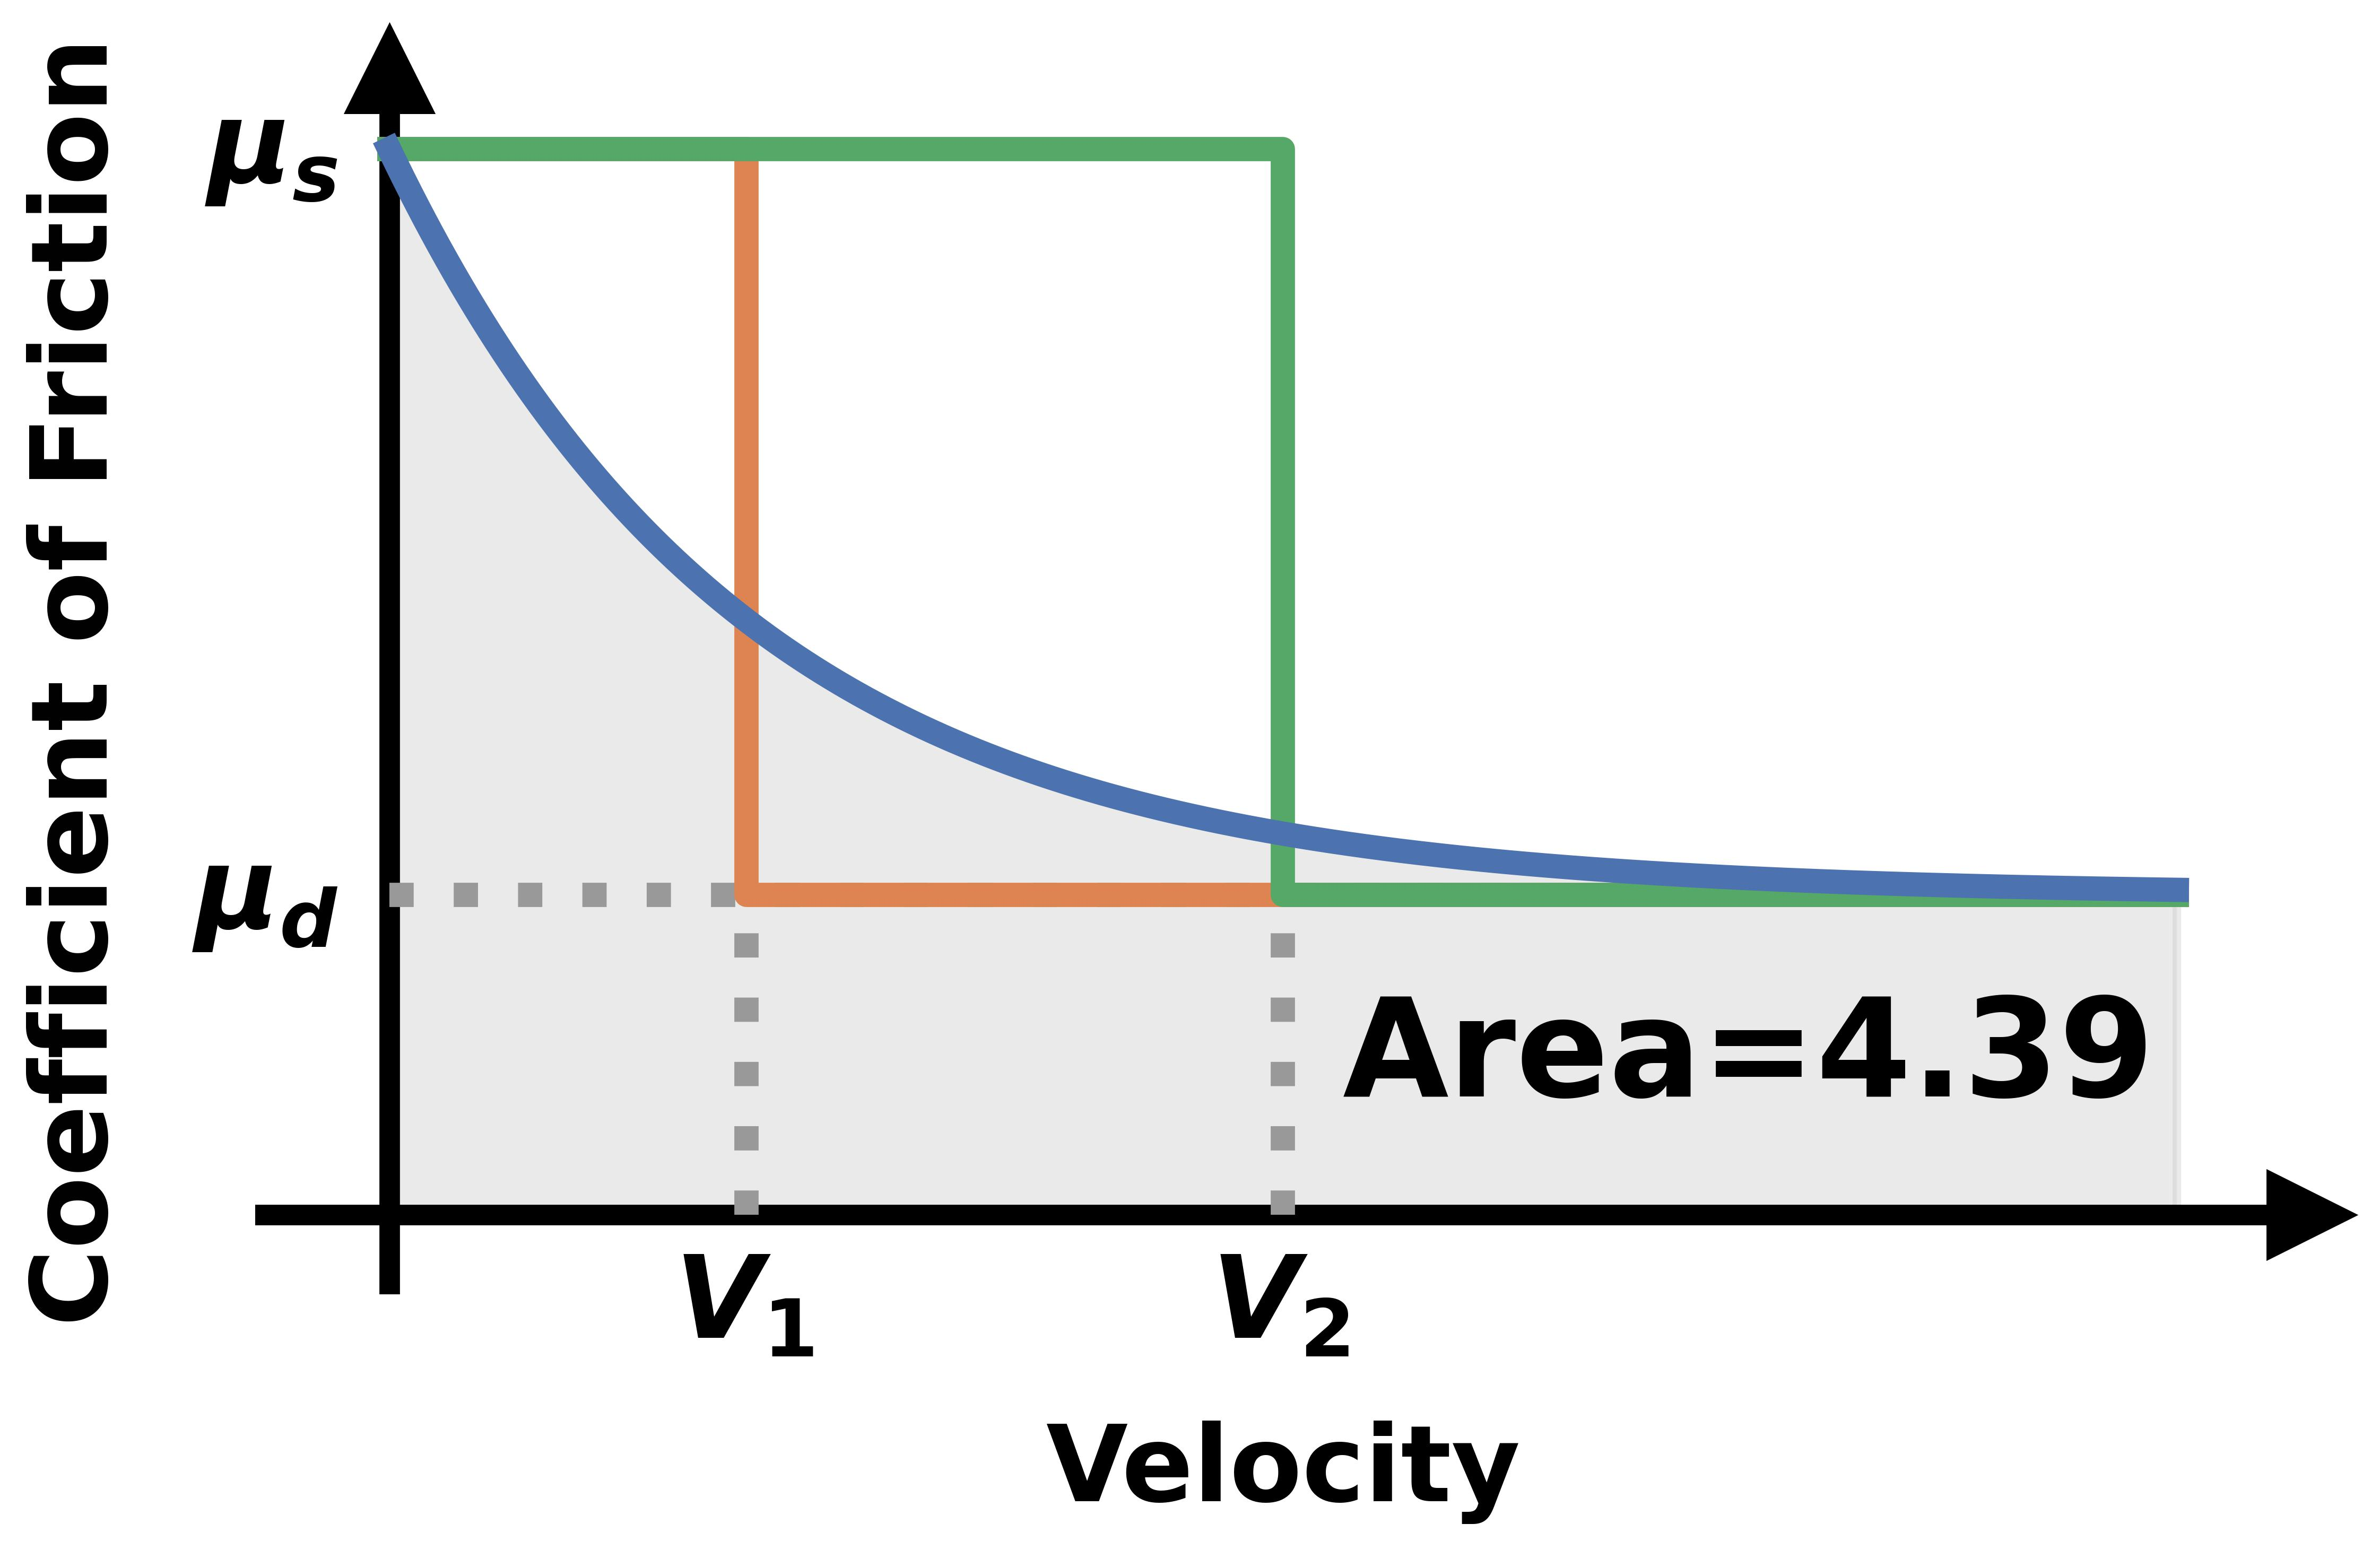
\includegraphics[width=\linewidth]{Stribeck_Coulomb_friction_filled_2}
				\subcaption{Stribeck friction curve with a critical velocity of $V_1$.}
				\label{fig:Stribeck_Coulomb_friction_filled_2}
			\end{minipage}
			\hfill
			\begin{minipage}[t]{0.325\linewidth}
				\centering
				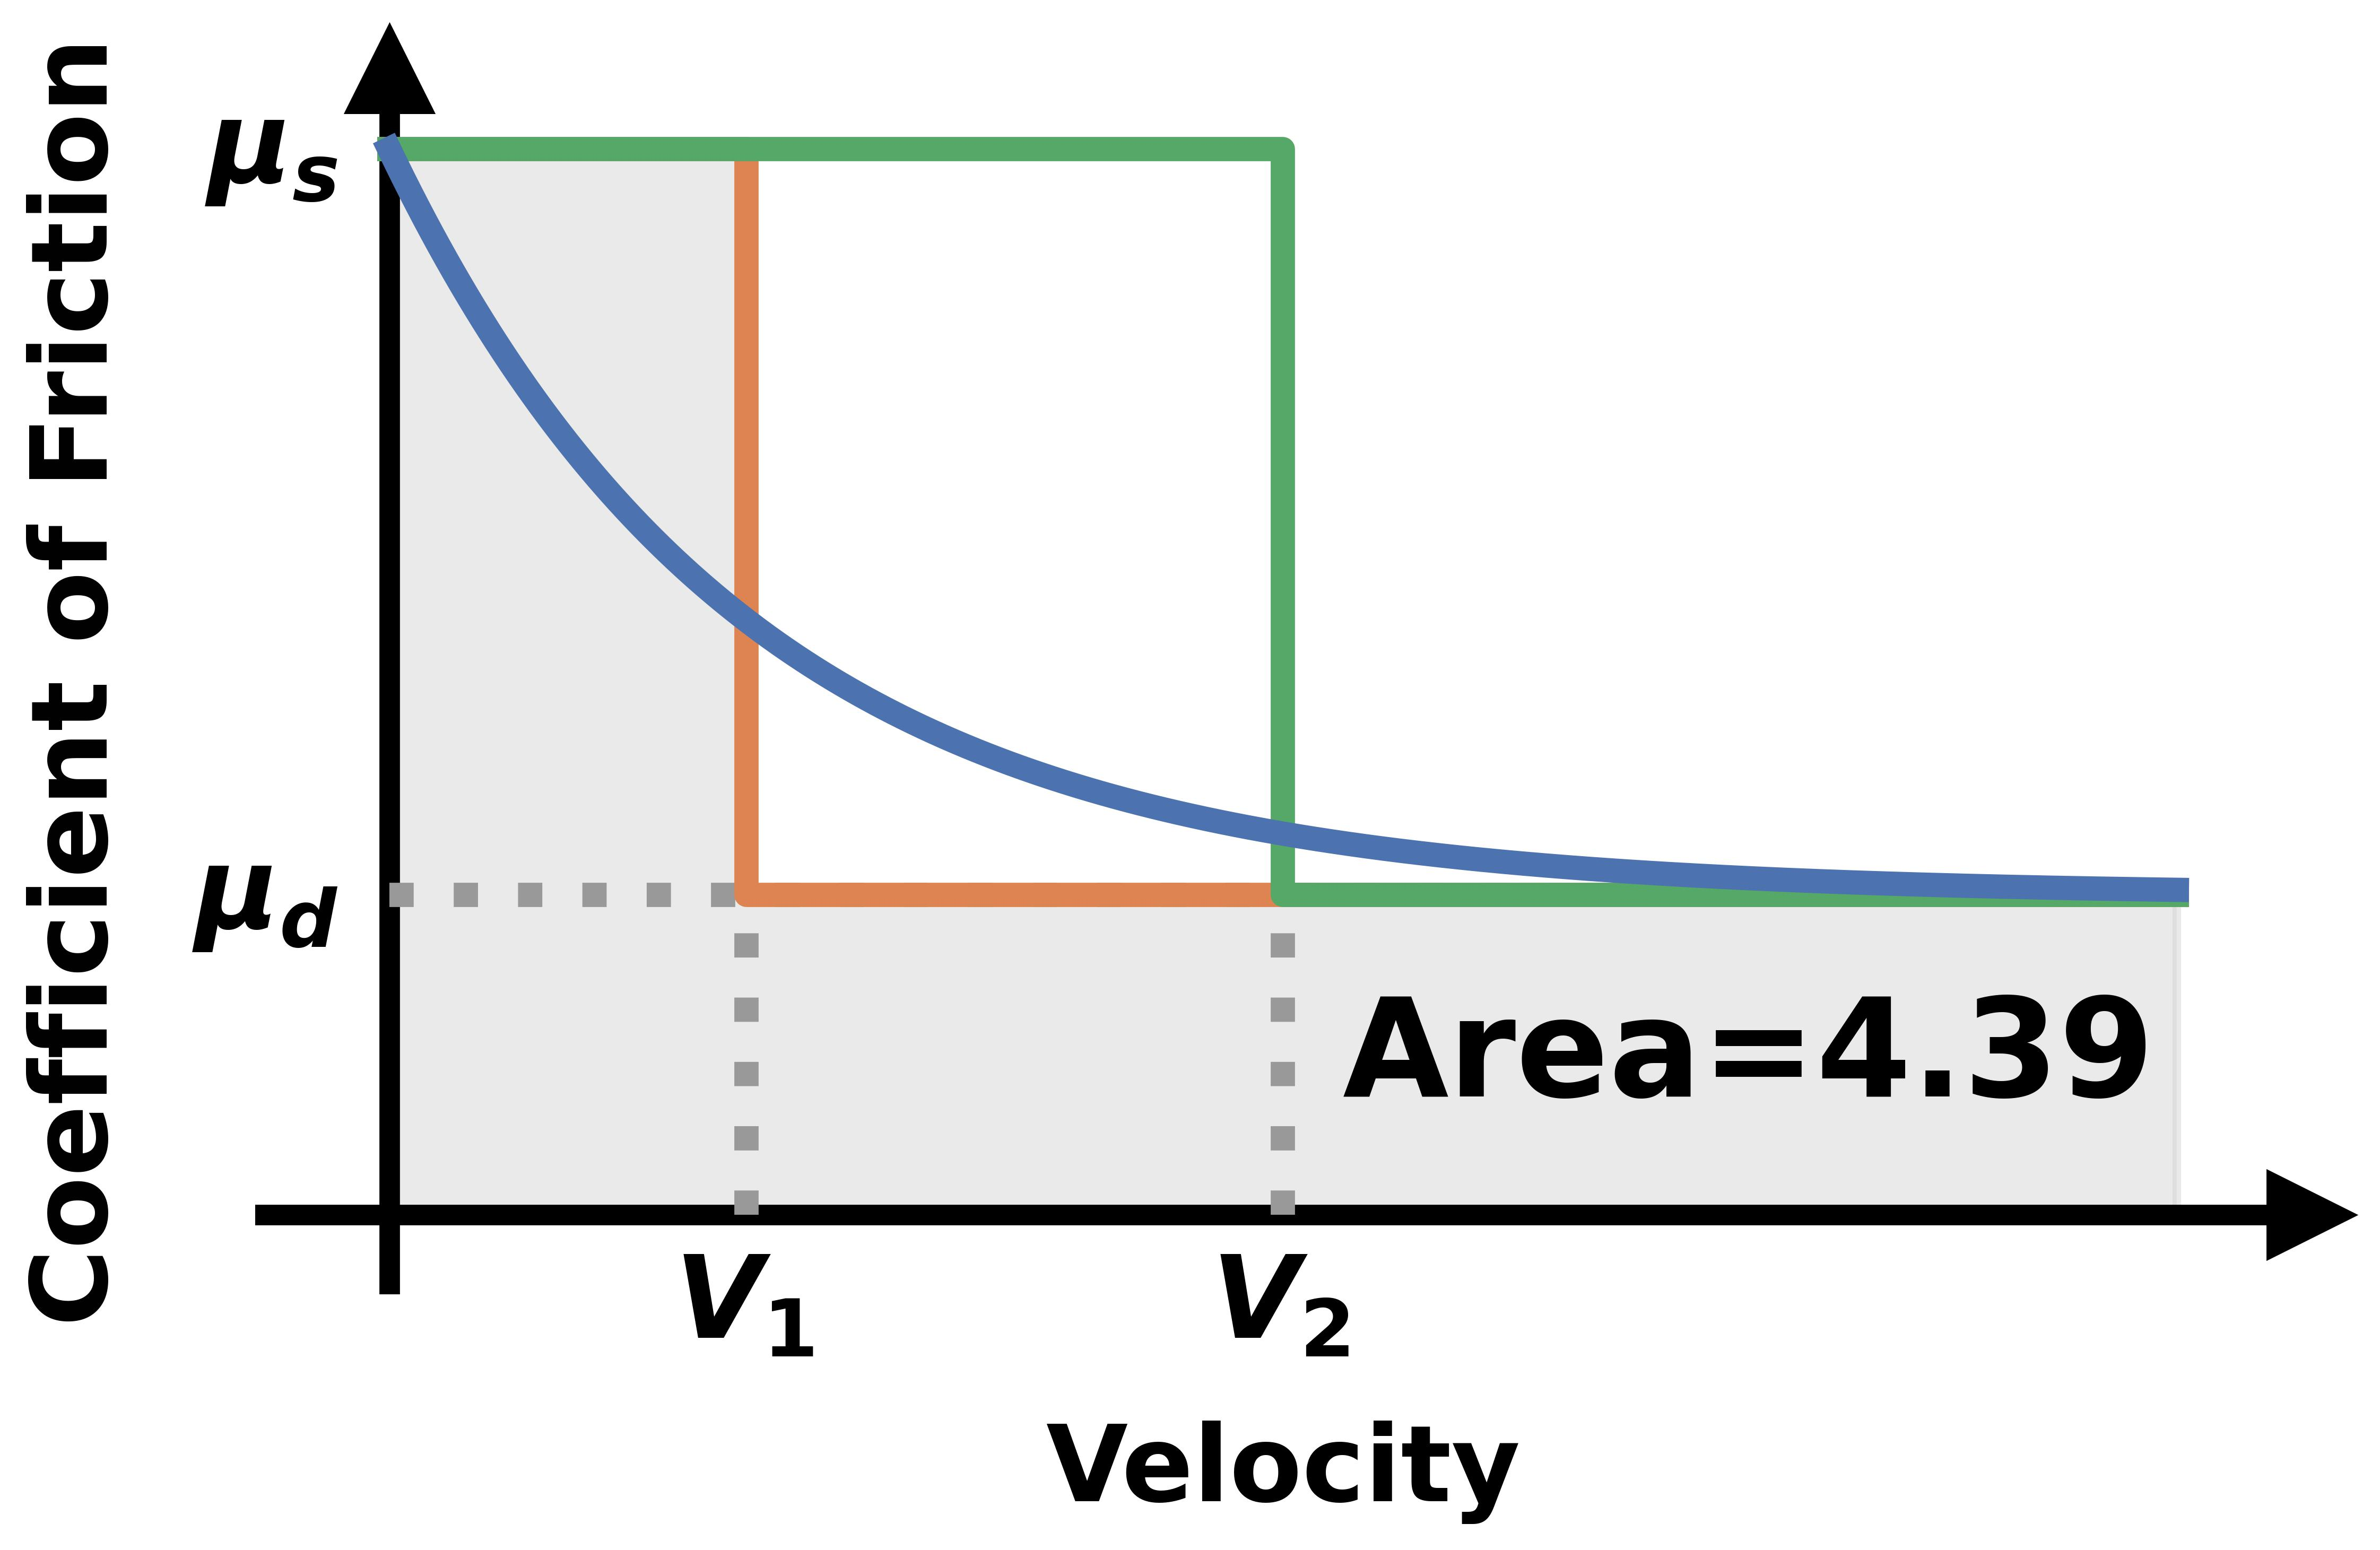
\includegraphics[width=\linewidth]{Stribeck_Coulomb_friction_filled_0}
				\subcaption{Coulomb friction curve with a critical velocity of $V_1$.}
				\label{fig:Stribeck_Coulomb_friction_filled_0}
			\end{minipage}
			\hfill
			\begin{minipage}[t]{0.325\linewidth}
				\centering
				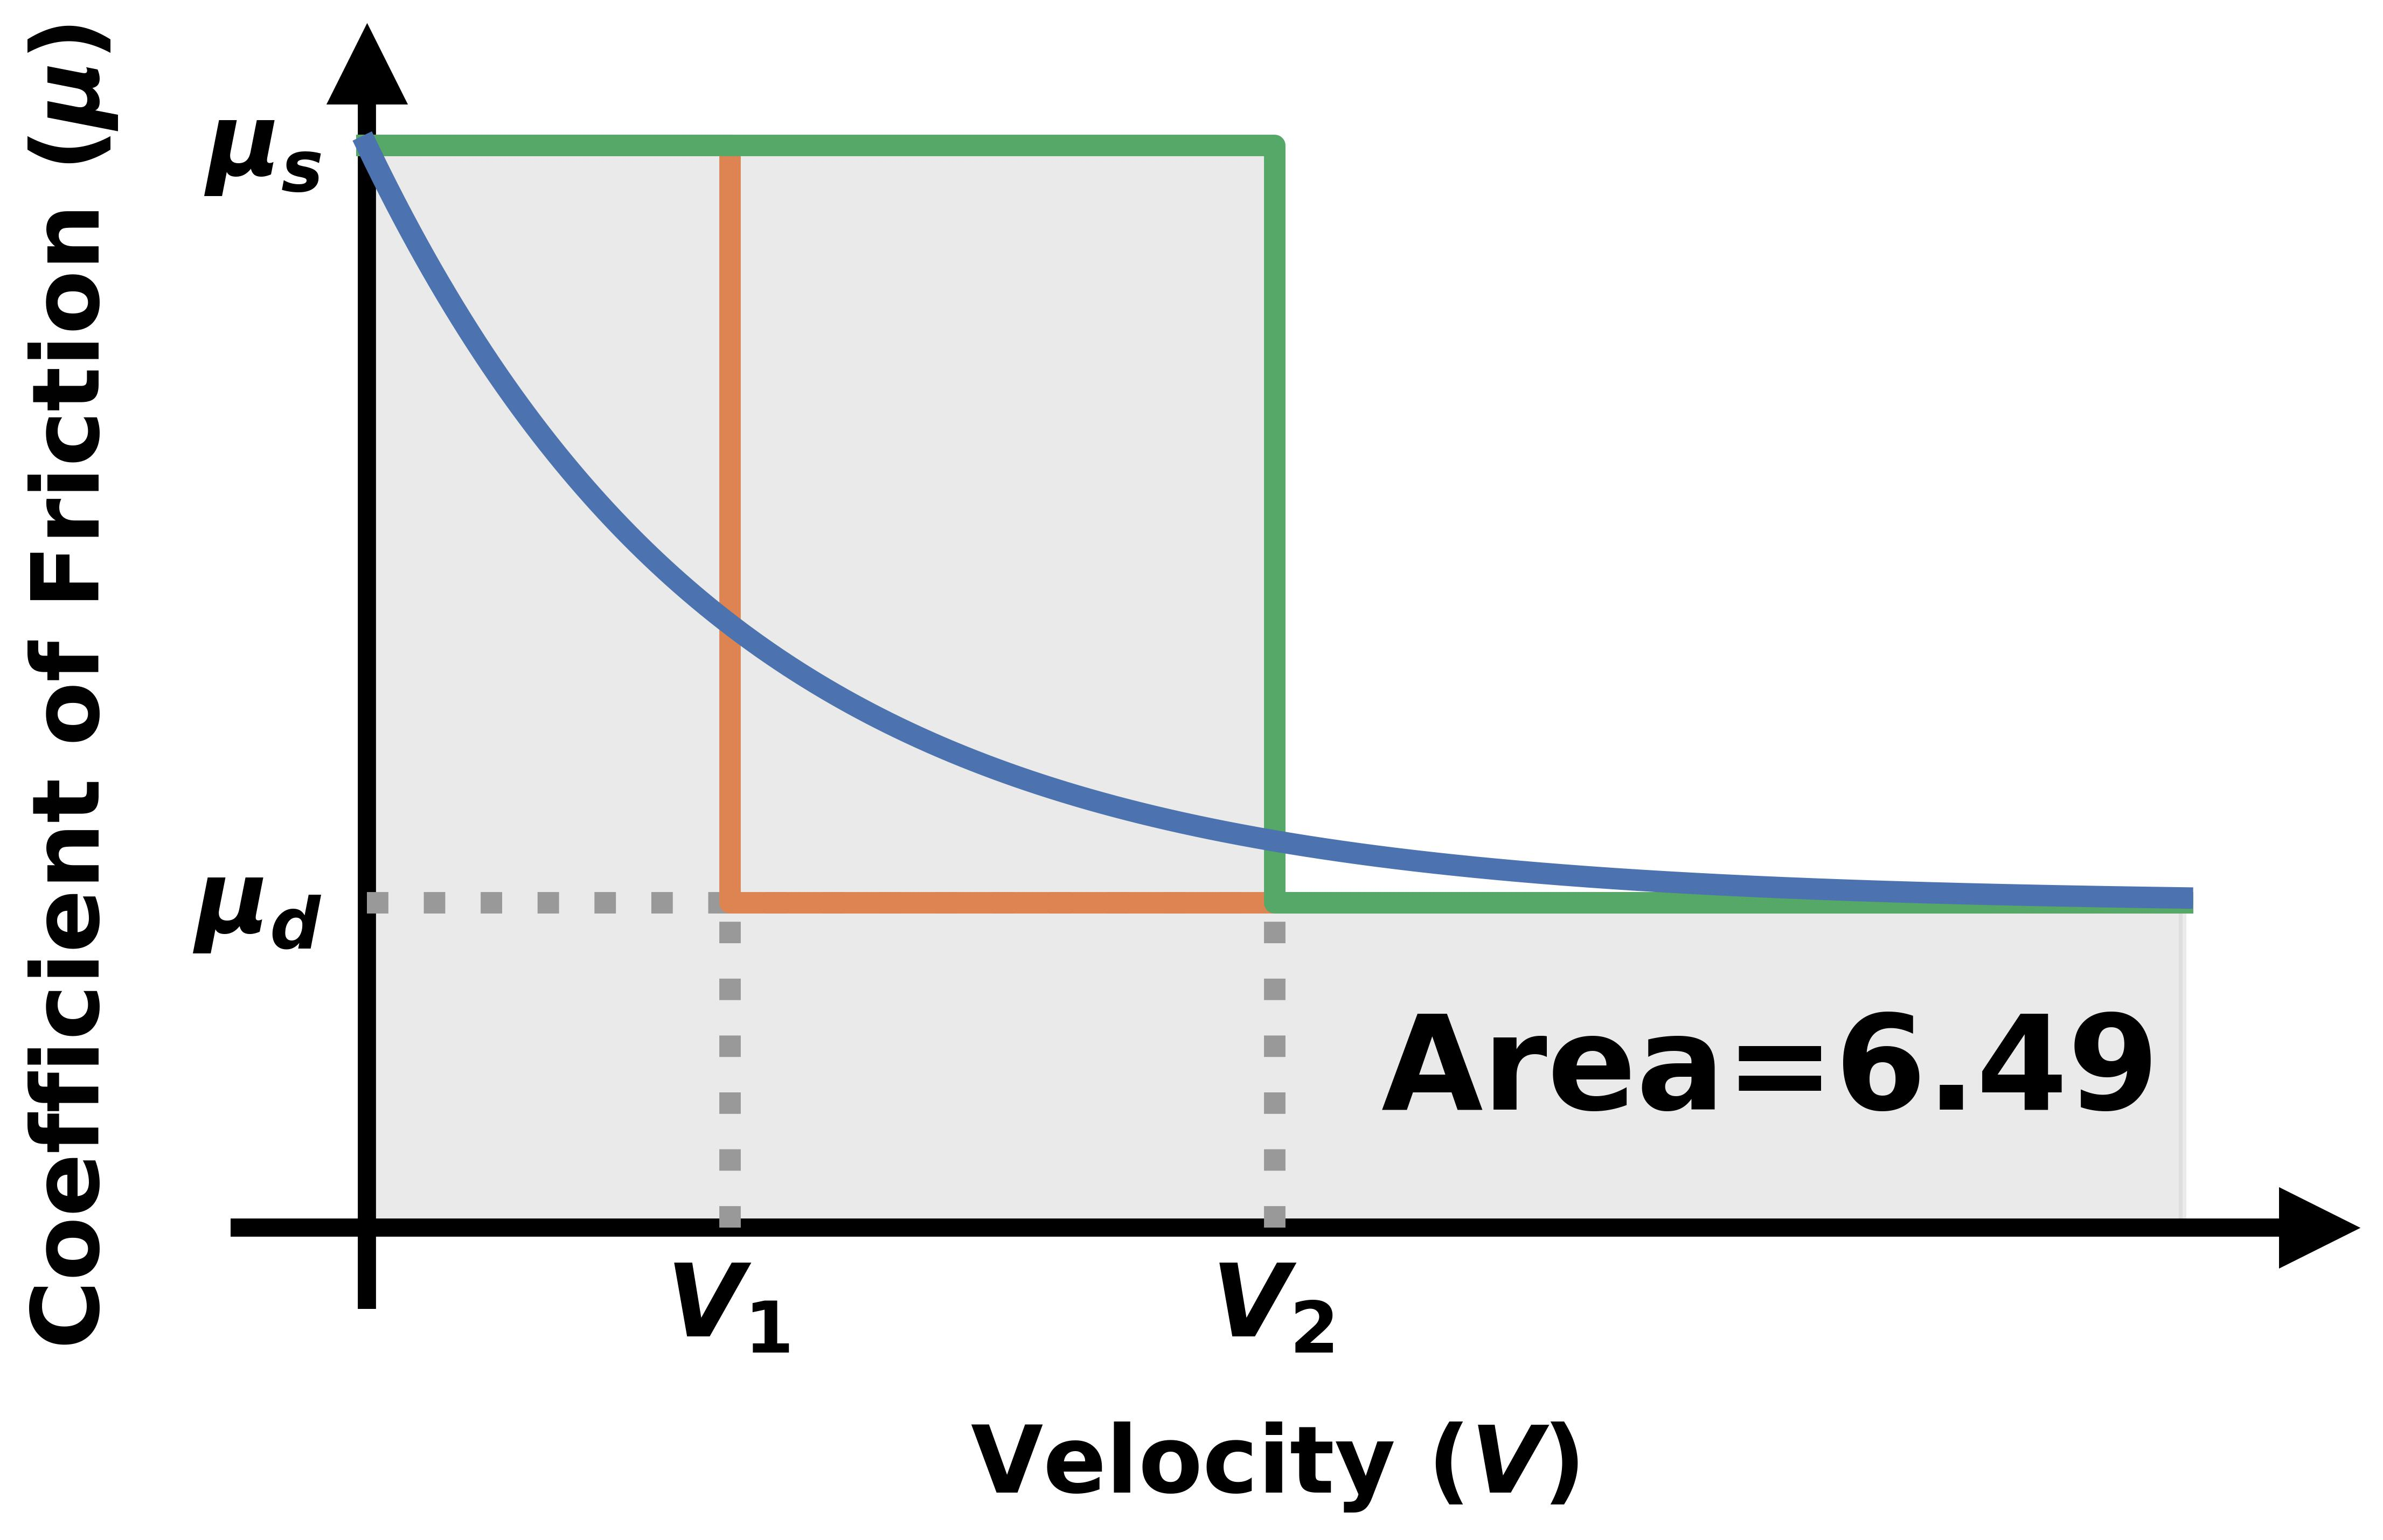
\includegraphics[width=\linewidth]{Stribeck_Coulomb_friction_filled_1}
				\subcaption{Coulomb friction curve with a critical velocity of $V_2$.}
				\label{fig:Stribeck_Coulomb_friction_filled_1}
			\end{minipage}
	\end{minipage}
	\caption[Areas under friction curves]{The areas under the friction curves are used as a measurement of how close the curves are to each other.  The choice of $V_1$ for the critical velocity of the Coulomb friction creates an area under the curve which is closer to the Stribeck curve.  The areas were calculated for the velocity range of $[0, 2V_2]$.  The legend from \figurename~\ref{figure:stribeck_coulomb_friction} is applicable here as well.}
	\label{fig:frictionmodelareaundercurves}
\end{figure}
